Conducted experiments are based on obtained the Titan supercomputer log data that were used for the quantitative model. The following information was extracted from the log per job: i) arrival timestamp (time when the job was queued); ii) execution start timestamp (i.e., startTime); iii) completion timestamp (i.e., endTime); iv) the number of requested nodes (1 node = 16 cores in Titan); v) requested walltime.

As the first approach in analysis there were no separation of jobs from different projects, jobs were grouped only based on their sizes. Further analysis was applied on jobs from just one project to extend the potential applicability of our model.

\subsubsection{Analysis using log data of all projects} \label{sec-experiments-3-1}

The following analysis actions are applied:
\begin{itemize}
    \item all jobs are divided into categories according to the number of required nodes and the volume of walltime requested (every category corresponds to a particular Titan's bin, where \textit{bin} is a group of jobs that are treated equally);
    \item for each category the following values are calculated: the expected value and variance of random variables describing waiting time in the queue and the utilization achieved by a single job;
    \item obtained values were used as input data in equation for the quantitative model to calculate the probability that jobs of a given category will be able to utilize provided allocation in 3 months;
    \item job launching scheme: one stream and there is always one job in the queue.
\end{itemize}

The outcome of the performed analysis is presented by the set of 5 plots (one per Titan's bin) in Figure~\ref{fig-proj-all-probability-distr} (outperformed groups are highlighted at the legend). Log data was collected for the period from May 2017 to April 2018.

\begin{figure}
    \centering
    \begin{subfigure}{.5\textwidth}
        \centering
        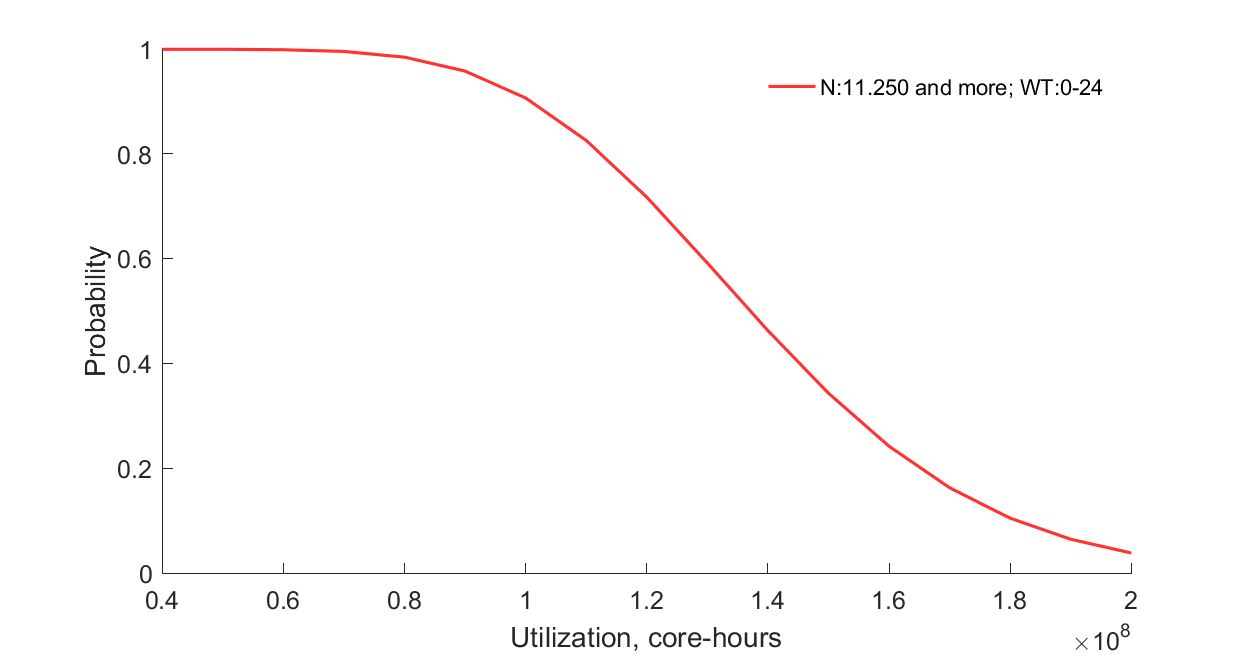
\includegraphics[width=.83\linewidth]{pics/proj-all-probability-distr-bin1.png}
        \caption{Bin-1 | nodes: [11,250:18,688]; walltime, h: [0:24]}
    \end{subfigure}
    \begin{subfigure}{.5\textwidth}
        \centering
        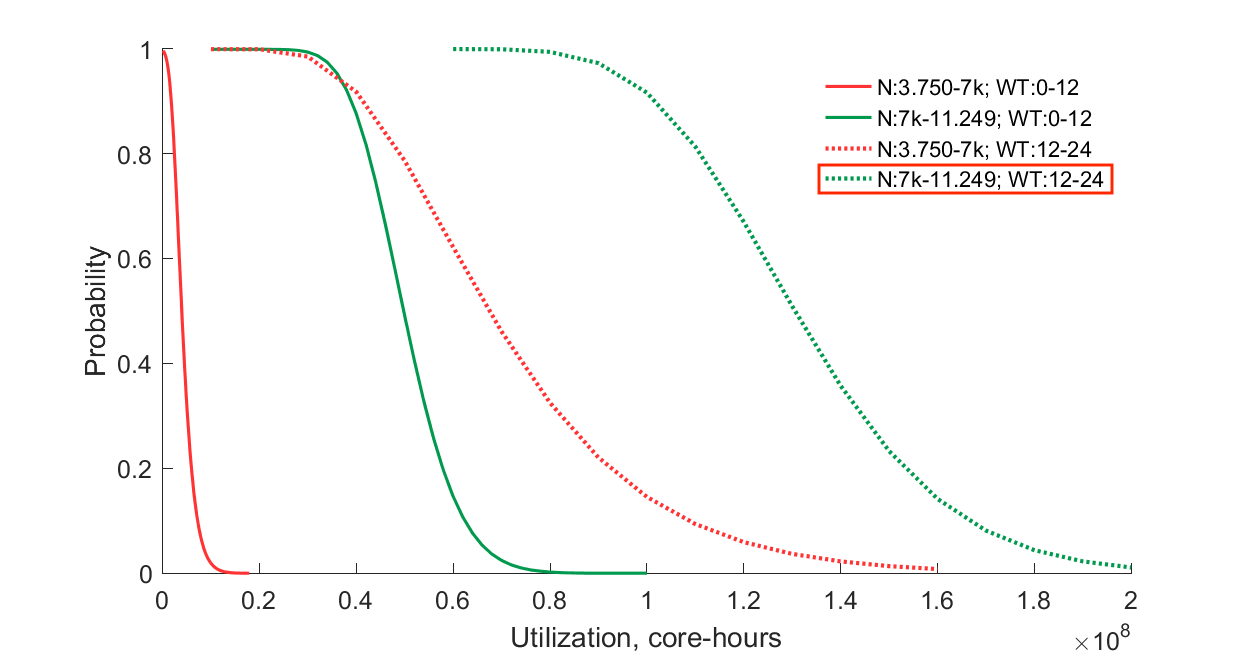
\includegraphics[width=.83\linewidth]{pics/proj-all-probability-distr-bin2.png}
        \caption{Bin-2 | nodes: [3,750:11,249]; walltime, h: [0:24]}
    \end{subfigure}
    \begin{subfigure}{.5\textwidth}
        \centering
        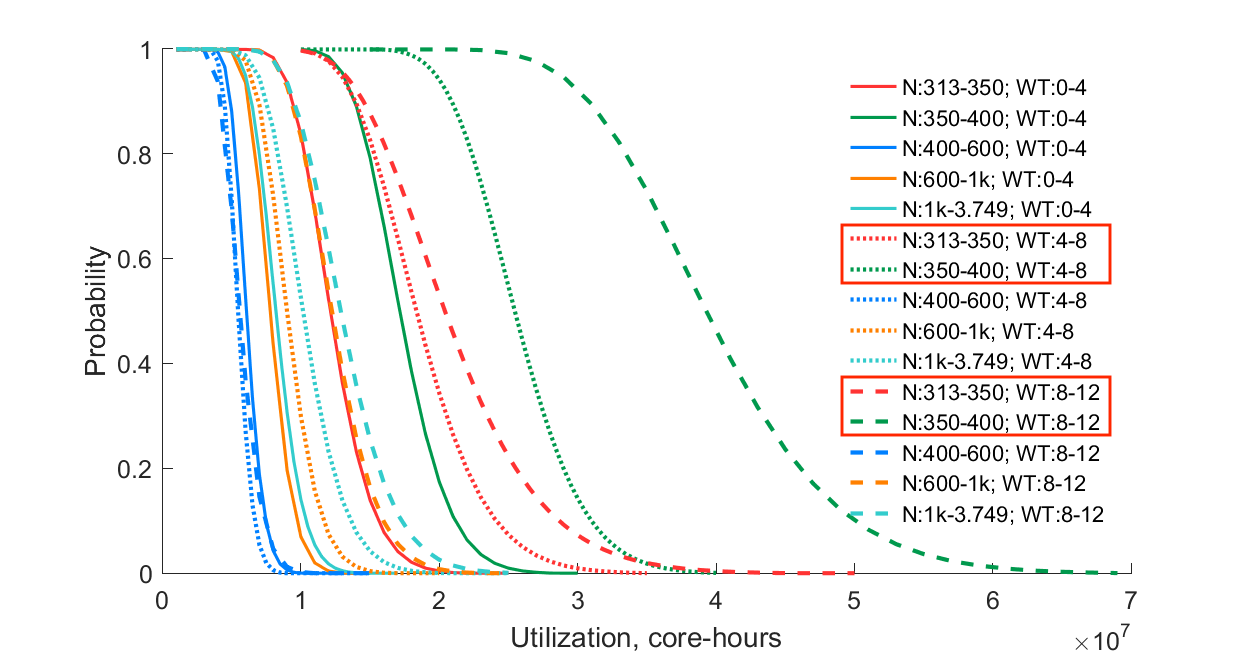
\includegraphics[width=.83\linewidth]{pics/proj-all-probability-distr-bin3.png}
        \caption{Bin-3 | nodes: [313:3,749]; walltime, h: [0:12]}
    \end{subfigure}
    \begin{subfigure}{.5\textwidth}
        \centering
        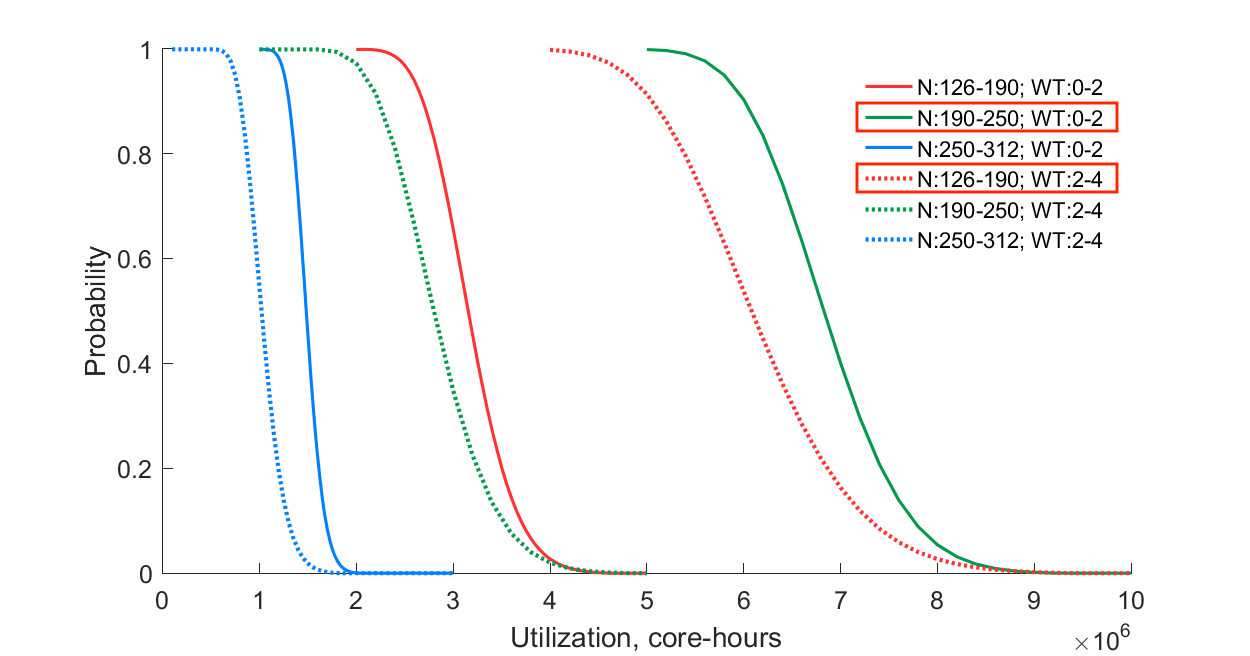
\includegraphics[width=.83\linewidth]{pics/proj-all-probability-distr-bin4.png}
        \caption{Bin-4 | nodes: [126:312]; walltime, h: [0:4]}
    \end{subfigure}
    \begin{subfigure}{.5\textwidth}
        \centering
        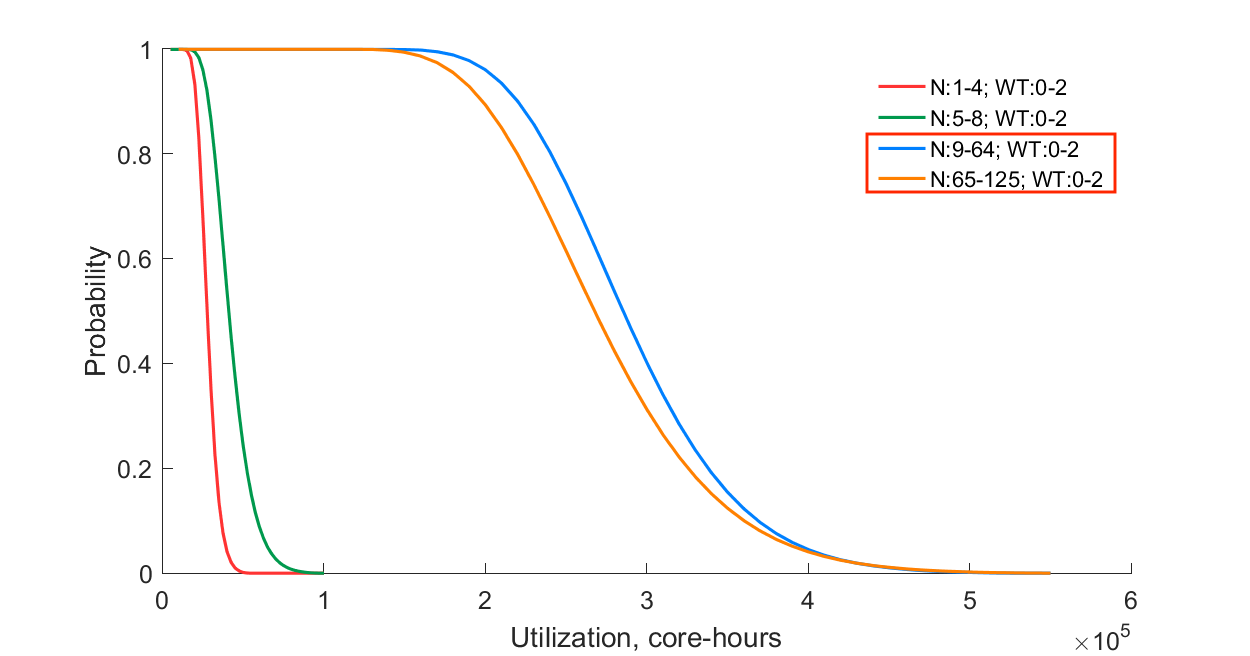
\includegraphics[width=.83\linewidth]{pics/proj-all-probability-distr-bin5.png}
        \caption{Bin-5 | nodes: [1:125]; walltime, h: [0:2]}
    \end{subfigure}
    \caption{Probability distributions of utilization of allocation time during 3 months per Titan's bins (based on Titan log data for 12 months)}
    \label{fig-proj-all-probability-distr}
\end{figure}

\subsubsection{Analysis using log data of one project (HEP110)} \label{sec-experiments-3-2}

Project HEP110 is associated with ALCC program, and computing jobs running under this project are from PanDA for the ATLAS experiment at LHC, CERN (actual ATLAS data wasn't in use for the current analysis, neither any data from PanDA). The outcome of the performed analysis for the project HEP110 is presented by the set of 2 plots (using jobs ``execution time'' and ``walltime''/``requested processing time'') in Figure~\ref{fig-hep110-probability-distr}.

\begin{figure}
    \centering
    \begin{subfigure}{.48\textwidth}
        \centering
        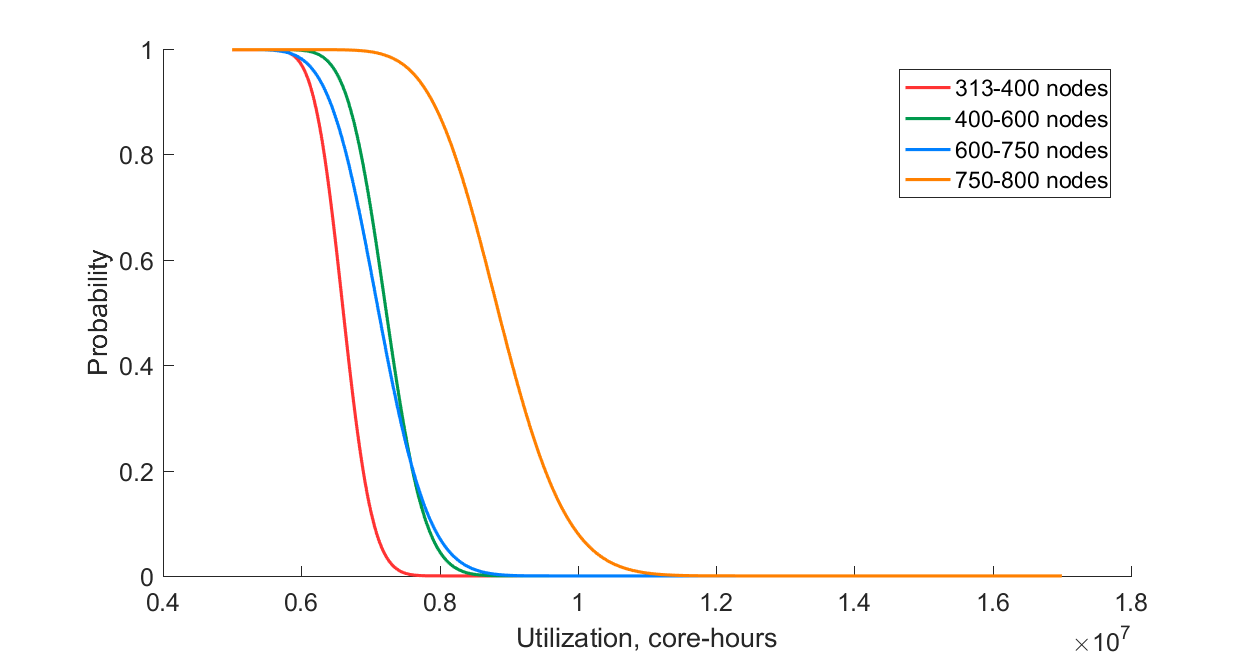
\includegraphics[width=.98\linewidth]{pics/hep110-probability-distr-exectime.png}
        \caption{Based on provided real execution time}
    \end{subfigure}
    \begin{subfigure}{.48\textwidth}
        \centering
        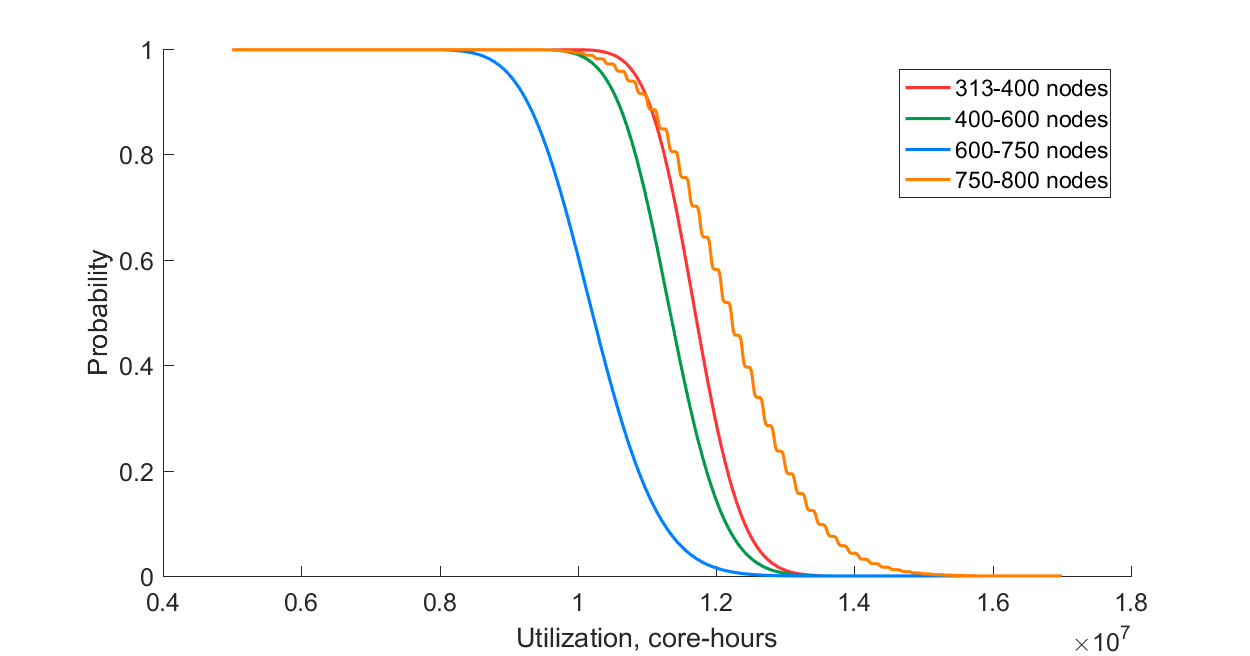
\includegraphics[width=.98\linewidth]{pics/hep110-probability-distr-walltime.png}
        \caption{Based on requested wall time}
    \end{subfigure}
    \caption{Probability distributions of utilization of allocation time during 3 months for HEP110 project at the Titan supercomputer (based on Titan log data for 6 months)}
    \label{fig-hep110-probability-distr}
\end{figure}
